\chapter{Огляд аналогових та цифрових датчиків}

\section{Загальні відомості про датчики температури}

% \thispagestyle{headings}

Спочатку потрібно розглянути загальні характеристики датчиків (вони у більшості своїй не належати до окремого типу датчиків).

Усі датчики можна поділити на два основних класи:

\begin{itemize}
    \item Пасивні датчики, які не потребують зовнішнього джерела живлення, і в залежності від взаємодії із зовнішнім середовищем генеруються електричний сигнал. Перевагами таких датчиків є те, що вони не мають вплив на зовнішнє середовище, мають низьку вартість, але водночас у таких датчиків складно встановити залежність між виміряним значенням (наприклад температурою) і напругою, потребують фільтрації шуму, що не завжди просто зробити.
    
    Прикладами таких датчиків є термопари, фотодіоди, п'єзоелементи, ультразвукові датчики відстані;
    \item Активні датчики, потребують зовнішнє джерело живлення -- сигнал збудження, такі датчики змінюють свої характеристики у відповідь на зміну зовнішніх сигналів, тобто перетворюють не електричні значення (температура) в опір, ємність або індуктивність. Вони простіші у зчитування значень. Прикладами таких датчиків є терморезистори, лазерні датчики відстані. 
\end{itemize}

Далі датчики можна поділити на наступні два підкласи:

\begin{itemize}
    \item Абсолютні, які вимірюють температуру чи будь-що без залежності від умов вимірів та зовнішнього середовища;
    \item Відносні -- результівний сигнал не показує точний стан вимірів, тобто потрібно додатково розрахувати ``правильне'' значення, в залежності від середовища та умов.
\end{itemize}

Знову ж таки, гарним прикладом таких підкласів є термопара та терморезистор: у той час, як у першому випадку на виході генерується відносний сигнал, який потрібно далі перерахувати беручи до уваги навколишню середу, опір терморезистор залежить тільки від температури.\\

\subsection{Аналогові та цифрові датчики}

За характеристикою результуючого сигналу датчики бувають аналогові та цифрові. Окремо взяті датчики з цих категорій, мають свої ``сильні'' характеристики, та область використання.

Так, аналогові датчики генеруються на виході неперервний електричний сигнал, який потрібно перетворити на дискретний за допомогою АЦП, і далі вже працювати з отриманим значенням для перетворення в одиницю вимірювання.

Своєю чергою, у цифрових датчиках вже присутня інтегральна мікросхема, яка перетворює вхідний сигнал, читати це значення вже можна за допомогою інтерфейсу, без або з мінімізацією подальших перетворювань. Калібрування таких датчиків часто робиться на виробництві.

Аналогові датчики забезпечують ширший діапазон вимірювання, наприклад термопара K типу, яка короткочасно без негативного впливу, може вимірювати температуру від $\ignorespaces -180^\circ~C$ до $\ignorespaces 1200^\circ~C$, але при цьому втрачає точність у деяких точках, має не ідеальну лінійну залежність, і є більше складним датчиком у використанні.

NTC термістор не може дати такий широкий спектр температур, але має надзвичайно високу швидкість реакції та є найдешевшим з датчиків.\\

\subsection{Характеристики датчиків}

При виборі датчика перш за все потрібно визначити потрібні вимоги до нього, в залежності від його подальшого застосування. Ці вимоги можуть бути описаними характеристиками, які присутні у datasheet потрібного датчика. Надзвичайно потрібно розуміти вимоги до датчика, адже ``ідеального'' датчика, під будь-які умови не існує.

Далі наведені найбільш типові характеристики датчиків і вимоги, які зазвичай вказуються в даташитах, або принаймні повинні бути вказані:

\begin{itemize}
    \item Робочий або динамічний діапазон деякої дії над датчиком (Input Full Scale), у разі температурних датчиків це, відповідно, температура, які можуть бути перетворені датчиком у напругу. Він є найвищим та найнижчим вхідним значенням, яке може бути застосовується до датчика, не викликаючи неприпустимо великої помилки або виходу датчика зі стану;
    \item Точність датчика, але взагалі позначається як можлива похибка. Похибка може бути як лінійна, мультиплікативна або нелінійна. У першому випадку вона постійна на всьому діапазоні виміру датчика, у другому збільшується при досягненні мінімального, або максимального значення, у третьому нелінійність на всьому діапазоні, у специфікації датчика часто вказуються графіки зміни точності.

    Процес калібрування датчиків може бути виконаний для підвищення точності та компенсації вище зазначених похибок;
    \item Роздільна здатність показує мінімальну зміну вимірюємої величини, яка призводить до зміни сигналу на виході. Аналогові датчики обмежені тільки роздільною здатністю АЦП;
    \item Робочий або динамічний діапазон датчика -- це інтервал значень вимірюваної величини, для якого датчик забезпечує прийнятні рівні точності та надійності;
    \item Функція перетворення -- це математична функція, яка визначає залежність вихідного сигналу датчика від вимірюваної фізичної величини (у цьому випадку, температури). Функція перетворення вказує, яким чином вихідний сигнал змінюється відповідно до зміни вхідної величини;
    \item Лінійність датчика -- показник того, наскільки точно функція перетворення може бути апроксимована лінійною функцією. Лінійний датчик легше калібрувати та використовувати;
    \item Час реакції, який потрібен датчику для виявлення та реакції на зміну вхідної величини.\\
\end{itemize}

\section{Вибір датчиків для експерименту}

Для порівняння були обрані наступні датчики (аналогові + цифрові) табл.~\ref{tab:comparison}. Саме така вибірка дозволить визначити як вибрати оптимальний датчик в залежності від цілі проєкту. Для отримання загального уявлення про методи вимірювання температури почнемо з аналогових датчиків: NTC терморезистора та термопари К-типу.

\begin{table}[h]
    \renewcommand{\arraystretch}{1.2}
    \caption{Порівняльна таблиця характеристик датчиків}
    \label{tab:comparison}
    \begin{tabular}{|M{3cm}|m{6cm}|m{6cm}|}
        \hline
        \textbf{Назва датчика} & \multicolumn{1}{c|}{\textbf{Базовий опис}} & \textbf{Основні характеристики} \\
        \hline
        NTC
        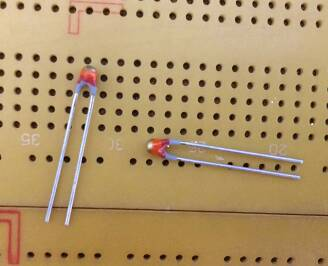
\includegraphics[width=\linewidth]{ntc.jpg}
        & Термістор, чутливий до зміни опору в залежності від температури. & Роздільна здатність: залежить від моделі, Робочий діапазон: від -50°C до +150°C, Протокол: аналоговий сигнал. \\
        \hline
        Термопара K типу
        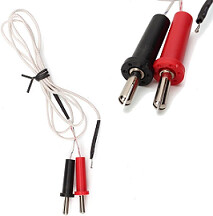
\includegraphics[width=0.7\linewidth]{thermocouple.jpg}
        & Складається з двох металевих провідників, генерує мікровольтовий сигнал при зміні температури на місці їх з'єднання. & Роздільна здатність: залежить від попарних металів -- 0.1°C, Робочий діапазон: від -270°C до +1372°C, Протокол: аналоговий сигнал. \\
        \hline
        DS18B20
        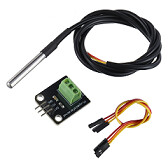
\includegraphics[width=0.77\linewidth]{ds18b20.jpg}
        & Цифровий температурний сенсор, випускається фірмою Maxim Integrated. & Роздільна здатність: 0.0625°C, Робочий діапазон: від -55°C до +125°C, Протокол: 1-Wire. \\
        \hline
        DHT11
        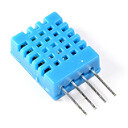
\includegraphics[width=\linewidth]{dht11.jpg}
        & Цифровий температурно-вологісний сенсор. & Роздільна здатність: 1°C, Робочий діапазон температури: від 0°C до 50°C, Протокол: спеціальний протокол на базі однопровідного інтерфейсу. \\
        \hline
        DHT22
        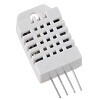
\includegraphics[width=\linewidth]{dht22.jpg}
        & Також відомий як AM2302, цифровий температурно-вологісний сенсор. & Роздільна здатність: 0.1°C, Робочий діапазон температури: від -40°C до +80°C, Протокол: спеціальний протокол на базі однопровідного інтерфейсу. \\
        \hline
        HTU21D
        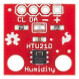
\includegraphics[width=0.6\linewidth]{htu21d1.jpg}
        & Цифровий температурно-вологісний сенсор, вироблений фірмою Measurement Specialties. & Роздільна здатність: 0.01°C, Робочий діапазон температури: від -40°C до +125°C, Протокол: I2C. \\
        \hline
    \end{tabular}
    \vspace{-3.3cm}
\end{table}

\clearpage

\section{Аналогові датчики}

\textbf{NTC терморезистор}\bigskip

Терморезистор, за своєю суттю резистор, який зроблений з напівпровідника та змінює свій опір зі зміною температури. Можна визначити два типи терморезисторів -- NTC терморезистор (термістор), який зменшує опір при нагріві (саме про них піде далі), та PTC терморезистор (позистор), який збільшує опір при нагріві. Є досить багато типів терморезисторів за формфактором, їх можна побачити на рис.~\ref{fig:thermoresistor_types}.

\begin{figure}[ht]
    \centering
    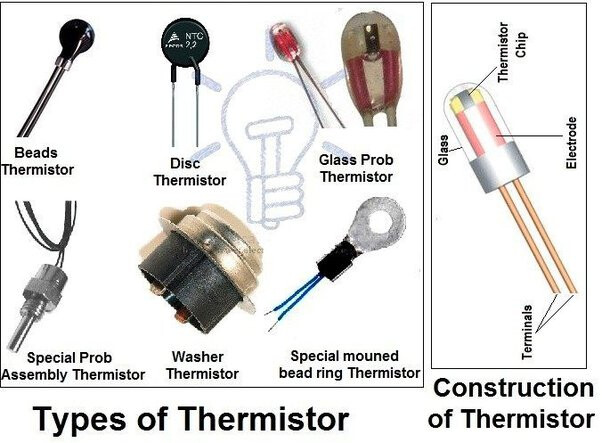
\includegraphics[width=0.7\linewidth]{thermoresistor_types.jpg}
    \caption{Різні типи терморезисторів}
    \label{fig:thermoresistor_types}
\end{figure}

На невеликому проміжку залежність опору від температури є лінійною, що дозволяє виконати апроксимацію використовуючи температурний коефіцієнт опору (TCR) для цієї області, та знаючи для якої референсної температури він відноситься (наприклад $25^\circ~C$) (рівняння \ref{eq:tcr}).

\begin{equation}
    \label{eq:tcr}
    \rho = \rho_0\left(1+\alpha\frac{t-t_0}{t_0}\right)
\end{equation}

На усьому робочому діапазоні залежність вже не лінійна, а отже розрахунки по такій формулі дадуть досить високу похибку на границях діапазону (рис.~\ref{fig:ntc_curve}).

\begin{figure}[ht]
    \centering
    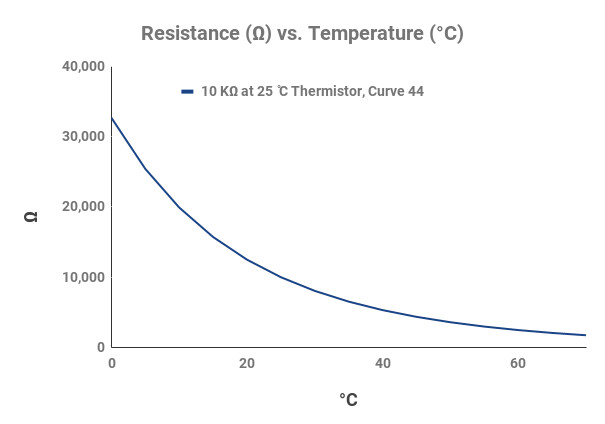
\includegraphics[width=0.9\linewidth]{ntc_curve.jpg}
    \caption{Характеристика NTC термістора}
    \label{fig:ntc_curve}
\end{figure}

Для деяких термісторів можна знайти специфікацію, у якій може бути надана таблиця залежності температури від опору з кроком 1°C або 5°C, проміжні значення можна розрахувати використовуючи лінійну інтерполяцію.

Зазвичай використовують іншу формулу для розрахунку температури з опору. Одним з параметрів, що характеризують залежність опору від температури, є коефіцієнт температурної реакції, що позначається $B$ та вимірюється у кельвінах. Цей коефіцієнт розраховується зі значень опору при двох конкретних температурах, і для багатьох термісторах може бути від 2600 до 4200K. У багатьох випадках ці температури вибирають 25°C і 100°C. Як правило, температури, використовувані при розрахунку коефіцієнта, задаються після букви, наприклад B25/100. Наступна експоненційна формула \ref{eq:ntc_beta} може бути використана для більш точних розрахунків.

\begin{equation}
    \begin{aligned}
        \text{R}_t = \text{R}_0 e^{\beta\left(\frac{1}{T}-\frac{1}{T_0}\right)}
        & \text{ , де T -- температура термістора} \\
        & \text{$T_0$ -- референсна температура} \\
        & \text{$\text{R}_0$ -- опір при референсній температурі} \\
        & \text{$\beta$ -- коефіцієнт температурної реакції}
    \end{aligned}
    \label{eq:ntc_beta}
\end{equation}

Окрім цього можна скористатися формулою Стейнхарта-Харта, яка дозволяє ще точніше розраховувати температуру, знаючи A, B, C коефіцієнти для взятого термістора (часто є у специфікації).

\begin{equation}
    \begin{aligned}
        \frac{1}{\text{T}} = A + B\ln(\text{R}) + C\left[\ln(\text{R})\right]^3
        & \text{ , де T -- температура у Кельвінах} \\
        & \text{R -- опір резистора}
    \end{aligned}
\end{equation}

\begin{figure}[ht]
    \centering
    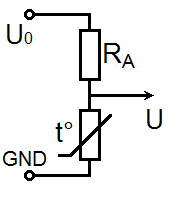
\includegraphics{ntc_connect.jpg}
    \caption{Схема підключення термістора}
    \label{fig:}
\end{figure}

Висновки по NTC термістру:

\begin{itemize}
    \item Сам по собі термістор має високу точність та малий час реакції, але без належного калібрування значення температури будуть відрізнятися на декілька градусів (особливо при зменшенні температури);
    \item Розрахунок температури можна зробити декількома способами: використовуючи рівняння, що на деяких мікропроцесорах буде сповільнювати роботу програми, або табличним способом, коли розраховуються значення температур в залежності від опору з деяким кроком, а проміжні значення отримуються за допомогою лінійної інтерполяції;
    \item Термістор вмикається в схему у верхнє або нижнє плече дільника напруги (від цього залежатиме вид характеристики). Зміна опору термістора призводить до зміни напруги дільника;
    \item Обираючи номінали дільника (резистора і термістора), слід врахувати, що струм, який протікає через термістор, спричиняє його нагрівання і, як наслідок, спотворення показань;
    \item Термістор один з найдешевших датчиків температури, що є великою перевагою.
\end{itemize}

\textbf{Термопара К-типу}\bigskip

Основною перевагою термопар є їх широкий температурний діапазон. Обмежена, по суті, абсолютним нулем (з нюансами) і температурою плавлення металів, тобто здатна робити виміри, де інші датчики просто вийдуть зі стану -- від -270 до + 1800$^\circ$C і вище.

Термопара досить цікавий датчик, адже в ній використовується інший ефект -- ефект Зеєбека, і на відміну від термістора, вона є пасивним датчиком, тобто створює дуже низьку напругу в залежності підвищення температури. Тут потрібно з'ясувати як саме вона працює.

Річ у тому, що при з'єднанні двох різнорідних сплавів провідників (наприклад Алюмель та Хромель) при їх нагріванні виникає різниці потенціалів, яка і генерує напругу. Нагрівати ми будемо так званий ``гарячий'' сплав, і зчитувати його напругу. Тут важливо зауважити, що інший -- ``холодний'' сплав, не можна нагрівати, адже саме при різних температурах виникає Електрорушійна сила, яка прямо пропорційно різниці цих температур. Термопара це відносний датчик, тому температура зовнішнього середовища до уваги не береться, важливі тільки відносини двох сплавів.

Як можна було зрозуміти, на виході (після перетворення) ми отримаємо температуру відносно холодного сплаву, а отже, щоб отримати реальну температуру на гарячому сплаві, потрібно завчасно виміряти температуру на холодному (референсному), для цього можна використати той же термістор. Цікаво, що цю проблему можна також вирішити помістивши холодний сплав у воду температури $0^\circ~C$, тоді компенсувати значення з гарячого сплаву не потрібно.

В залежності від потреб використовуються різні сплави, наприклад наша термопара К-типу використовує Алюмель (холодний) та Хромель (гарячий), і дозволяє вимірювати у досить широкому діапазоні, з кінцевими границями у $-200^\circ~C$ -- $1260^\circ~C$, таку термопару зручно використовувати для термостата у паяльні станції. Термопара Е-типу складається з Хромелю та Константану, і дозволяє вимірювати дуже низькі температури, не піддається корозії, і тому може бути використана у вологих середовищах. Також використовуються наступні сплави: E (хромель-константант), J (залізо-константант), K (хромель-алюмель), M (мідно-копель), N (ніхросил-нісил) та інші.

Як було сказано вище, термопара генерує низьку напругу, К-типу -- 0.4мВ/$^\circ$C, АЦП з роздільною здатністю 10 бітів не здатен зчитати таку напругу, тому її потрібно спочатку підсилити за допомогою неінвертуючого підсилювача, про це більш детально у практичній частині.

Для перетворення значення з підсиленого виходу термопари у температуру скористуємося наступною формулою \ref{eq:thermocouple}.

\begin{equation}
    \label{eq:thermocouple}
    \begin{aligned}
        T = \frac{V}{Ga} + T_{\text{ref.}}
        & \text{ , де V -- підсилений сигнал} \\
        & \text{G -- коефіцієнт підсилення} \\
        & \text{$\alpha$ -- коефіцієнт Зеєбека, табличне значення} \\
        & \text{$T_{\text{ref.}}$ -- температура холодного сплаву}
    \end{aligned}
\end{equation}

\begin{figure}[ht]
    \centering
    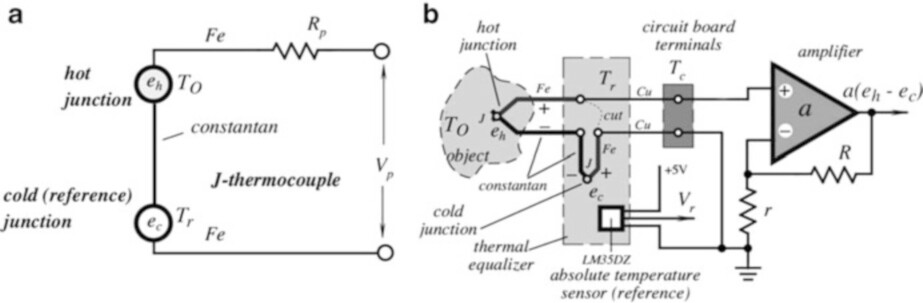
\includegraphics[width=\linewidth]{thermocouple_usage.jpg}
    \caption{Приклад використання термопари}
    \label{fig:thermocouple_usage}
\end{figure}
%\FloatBarrier

Висновки по термопарі К-типу:

\begin{itemize}
    \item Більше ніяких складних формул, у термопарі К-типу ми маємо лінійну залежність 0.4мВ/$^\circ$C вище нуля, все що потрібно це підсилити цю напругу та скористатися простою формулою;
    \item Термопара має нижчу швидкість реакції, а той же час здатна вимірювати високі температури;
    \item Має непогану точність, але її складно досягти, без ізоляцій і фільтрів на входах та виходах. Термопара К-типу має майже лінійну залежність, тому калібровка не є складно. Ці нюанси не такі вже і важливі, адже термопарою вимірюють високі температури, де похибка у декілька градусів не страшна.\\
\end{itemize}


\section{Цифрові датчики}

З попередньої частини про аналогові датчики можна було з'ясувати, що працювати з ними важко, потрібно використовувати складні формули для перетворення напруги в одиниці вимірювання температури, часто потрібно використовувати фільтри сигналу, щоб запобігти значного спотворення сигналу доки він дійде до АЦП. У випадку с термопарою ситуація виходить ще складніша, адже окрім фільтрації потрібно ще знати температуру холодного сплаву, і додавати її або програмним способом, або просто у схемі з'єднавши послідовно термопару та схему компенсації, яка повинна генерувати напругу з тим же шагом (0.4мВ/$^\circ$C) (рис.~\ref{fig:thermocuple_cold_junction_compensation}).
\enlargethispage{\baselineskip}

\begin{figure}[ht]
    \centering
    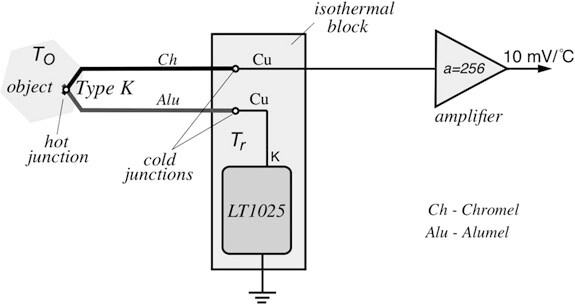
\includegraphics[width=0.8\linewidth]{thermocouple_cj_compensation.jpg}
    \caption{Додавання сигналів з термопари та компенсатора холодного сплаву}
    \label{fig:thermocuple_cold_junction_compensation}
\end{figure}

Ці недоліки, коли потрібна максимальна простота з боку схемотехнічної реалізації та надійність, яку дає виробник, приводить нас до цифрових датчиків. Вони містять у собі АЦП, інтегральну мікросхему, фільтри, і на виході генерують дискретний сигнал, який передають по спеціальних шинах даних стійких до завад (принаймні, на малій відстані). Існує безліч цифрових датчиків, про деякі з них піде річ далі.\\

\textbf{DS18B20}\bigskip

Один з найпопулярніших цифрових датчиків температури, який виробляється фірмою Maxim Integrated. Передача даних відбувається за допомогою пропрієтарної дуплексної шини даних 1-Wire, яка використовує одну лінію для взаємодії з підключеними девайсами. На шину можна під'єднати безліч датчиків, адже кожен з них має свій унікальний номер. Датчик потребує живлення 5В, яке також може подаватися через шину дану (паразитне живлення). Шину даних потрібно підтягнути до живлення резистором ~5 кОм. На рис.\ref{fig:ds18b20_scheme} зображена внутрішня реалізація датчику.

\begin{figure}[ht]
    \centering
    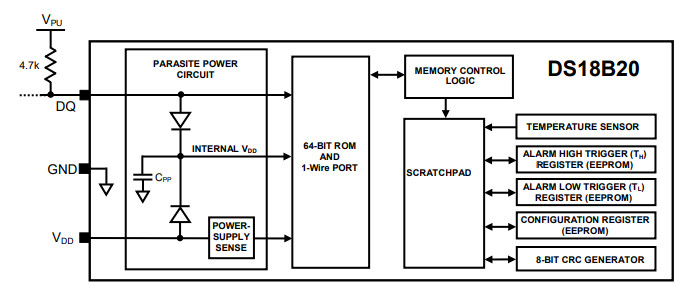
\includegraphics[width=\linewidth]{ds18b20_scheme.jpg}
    \caption{Внутрішня структура DS18B20}
    \label{fig:ds18b20_scheme}
\end{figure}

Датчик здатен вимірювати температуру у діапазоні від -55$^\circ$C до 125$^\circ$C з точністю 0.5$^\circ$C. Роздільну здатність можна також налаштувати від 9 до 12 бітів (за замовчуванням 12), тобто, наприклад 11 бітів відповідають {$\frac{125-(-55)}{2^{11}}~\approx~0.09^\circ$C} ``чутливості''. За специфікацією маємо наступні калібровані значення: 0.5$^\circ$C, 0.25$^\circ$C, 0.125$^\circ$C, 0.0625$^\circ$C. Щобільше обрана розрядність, то повільніше буде вимірювати температуру датчик: 93.75 мс, 187.5 мс, 375 мс, 750 мс.

Після посилання команди на вимір температури, в залежності від розрядності, вимір займе вищевказаний час. Датчик зберігає температуру у 16 бітний регістр, який після вимірювання потрібно зчитувати.

\begin{figure}[ht]
    \centering
    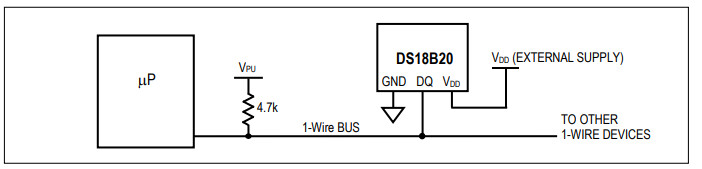
\includegraphics[width=\linewidth]{ds18b20_connect.jpg}
    \caption{Приклад підключення датчика}
    \label{fig:}
\end{figure}

В цілому цей датчик має низьку ціну, дозволяє за допомогою інтерфейсу 1-Wire організувати мережу датчиків, що охоплюють ту чи іншу область. Наприклад, декілька датчиків можна встановити у теплиці та контролювати температуру. Взагалі, саме такі проєкти є головними споживачами цього датчика.\\

\textbf{DHT11}\bigskip

На відміну від попереднього датчика цей є більше простим, але окрім темеператури дозволяє вимірювати вологість. Передача даних відбувається за допомогою однопровідної шини даних використовуючи простий протокол для комунікації. Не підтримує під'єднання декількох датчиків на одну шину.

Може працювати від напруги 3.3 до 5 В. Шина даних підтягується до живлення резистором ~5 кОм. Для вимірювання температури використовує термістор, а коефіцієнти калібрування записані на read-only OTP пам'яті. Точність DHT11 зазвичай становить +/-2$^\circ$C для температури та +/- 5\% для вологості. Роздільна здатність -- 1$^\circ$C. Резистивний елемент, вбудований у датчик, реагує на зміни вологості.

У цьому датчику не має вбудованої пам'яті для збереження результатів вимірювань, а час вимірювання становить 2 секунди, а у найгірших випадках до 30 секунд.

\begin{figure}[ht]
    \centering
    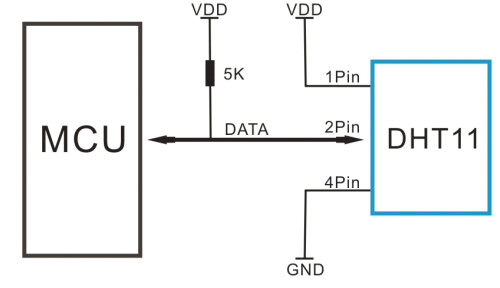
\includegraphics[width=0.6\linewidth]{dht11_connect.jpg}
    \caption{Приклад підключення датчика}
    \label{fig:}
\end{figure}

Взагалі, датчик можна вважати невдалим, і його використання навіть у проєктах теплиці є великим питанням. Має низьку ціну, але водночас усі його характеристики є поганими, порівнюючи з іншими датчиками. Не рекомендується для використання.\\

\textbf{DHT22}\bigskip

Датчик DHT22, також відомий як AM2302, є вдосконаленою версією DHT11, надаючи покращену точність та ряд інших характеристик для вимірювання температури та вологості. Для передачі даних DHT22 використовує простий цифровий інтерфейс, але у порівнянні з DHT11, має меншу частоту оновлення даних, що робить його більш стійким до зовнішніх перешкод.

Побудований також на базі термістора, використовує конденсаторні елементи для вимірювання вологості. Зміна вологості впливає на діелектричні властивості конденсаторів, що визначається мікроконтролером для визначення вологості повітря. На відміну від DHT11 використовує шкалу компенсації температурних змін, що дозволяє коригувати вимірювання вологості в залежності від змін температури, щоб забезпечити точніші результати в різних умовах. Також має певну стійкість до зовнішніх впливів, таких як конденсація водяної пари.

DHT22 вимірює температуру від -40 до 80$^\circ$C та вологість від 0\% до 100\%. Точність DHT22 зазвичай становить +/- 0.5$^\circ$C для температури та +/- 2\% для вологості. Роздільна здатність - 0.1$^\circ$C.

Таким чином, DHT22 є більш розвиненою версією DHT11. Він має вищу точність вимірювань, а також можливості компенсації температурних змін.\\

\textbf{HTU21D}\bigskip

Датчик HTU21D1 є цифровим датчиком вологості та температури, розробленим компанією Measurement Specialties. Він відзначається високою точністю вимірювань та компактним дизайном.

Для передачі сигналу у цифровому сигналі використовує шину I²C, що дозволяє дуже просто його підключати та використовувати багато пристроїв на єдиній шині. Датчик має низьке енергоспоживання (максимальна напруга -- 3.8В, струм у стані спокою -- 0.02 мкА, у стані вимірювання -- до 500 мкА) та є більш чутливим до змін температури. Має високу точність вимірювань. Точність для вологості може сягати до +/- 2\%, а для температури -- до +/- 0.3°C. Не потребує калібрації, адже кожен датчик індивідуально калібрується і тестується. Номер партії друкується на датчику, а його власний ідентифікатор зберігається на мікросхемі, який можна зчитати за допомогою команди. Роздільна здатність може бути змінена за допомогою команди (11 -- 14 бітів для температури та 8 -- 12 для вологості). Тобто роздільна здатність при максимальній розрядності 12 бітів отримаємо роздільну здатність ~ 0.01$^\circ$C.

Датчик забезпечує вимірювання вологості в діапазоні від 0\% до 100\% та температури від -40°C до 125°C. Датчик має вбудований нагрівний елемент, який здатен підвищити температуру на 1.5$^\circ$C. Як і попередній датчик здатен компенсувати температуру при вимірюванні вологості від 0 до 80$^\circ$C.

На відміну від усіх попередніх цифрових датчиків, час виміру температури не перевищує 50 мс при максимальній роздільній здатності.

Специфікація надає формули для виміру приблизної точки роси використовуючи зчитану температуру та вологість (формули \ref{eq:dew_point1}-\ref{eq:dew_point2})

\begin{equation}
    \begin{aligned}
        PP_{Tamb} = 10^{\left[A-\frac{B}{\left(T_{Amb}+C\right)}\right]}
        & \text{ , де T -- виміряна температура} \\
        & \text{A, B, C -- константи 8.1332, 1762.39, 235.66}
    \end{aligned}
    \label{eq:dew_point1}
\end{equation}

\begin{equation}
    \begin{aligned}
        T_d = -\left[\frac{B}{\log_{10} \left(RH_{amb}\cdot\frac{PP_{Tamb}}{100}\right)-A}+C\right]
        & \text{ , де $T_d$ -- точка роси} \\
        & PP_{Tamb} \text{ -- парціальний тиск} \\
        & RH_{amb} \text{ -- вологість повітря}
    \end{aligned}
    \label{eq:dew_point2}
\end{equation}


